% gm-04-SystemsEquations.tex

\documentclass[xcolor=dvipsnames]{beamer}

\usepackage{cancel}
\renewcommand{\CancelColor}{\color{red}}
\usepackage{graphicx}
\usepackage{wrapfig}
\usepackage{colortbl}
\usepackage{color}
\usepackage{alltt}
\usepackage{media9}
\renewcommand*{\thefootnote}{\fnsymbol{footnote}}
\definecolor{myblue}{rgb}{0.8,0.85,1}

\mode<presentation>
{
  \usetheme{Warsaw}
  \setbeamercovered{transparent}
}
% \usecolortheme[named=OliveGreen]{structure}
\setbeamertemplate{navigation symbols}{} 
\setbeamertemplate{blocks}[rounded][shadow=true] 

% this is for overlaying math symbols, see https://tex.stackexchange.com/questions/12895/overlay-symbol-with-another
\def\qeq{\mathrel{%
    \mathchoice{\QEQ}{\QEQ}{\scriptsize\QEQ}{\tiny\QEQ}%
}}
\def\QEQ{{%
    \setbox0\hbox{$\longrightarrow$}%
    \rlap{\hbox to \wd0{\hss/\hss}}\box0
  }}

\newcounter{expls}
\setcounter{expls}{0}
\newcommand{\beispiel}[1]{\refstepcounter{expls}\textbf{Example \arabic{expls}: #1.}}

\newcounter{exercise}
\setcounter{exercise}{0}
\newcommand{\ubung}[0]{\refstepcounter{exercise}\textbf{Exercise \arabic{exercise}: }}

\newif\ifBCITCourse
\BCITCoursetrue
% \BCITCoursefalse
\newif\ifWhichCourse
\WhichCoursetrue
\WhichCoursefalse
\ifBCITCourse
\ifWhichCourse
\newcommand{\CourseName}{Technical Mathematics for Food Technology}
\newcommand{\CourseNumber}{MATH 1441}
\newcommand{\CourseInst}{BCIT}
\else
\newcommand{\CourseName}{Technical Mathematics for Geomatics}
\newcommand{\CourseNumber}{MATH 1511}
\newcommand{\CourseInst}{BCIT}
\fi
\else
\newcommand{\CourseName}{Philosophy and Literature}
\newcommand{\CourseNumber}{PHIL 375}
\newcommand{\CourseInst}{UBC}
\fi

\title{Systems of Linear Equations}
\subtitle{{\CourseNumber}, BCIT}

\author{\CourseName}

\date{September 18, 2017}

\begin{document}

\begin{frame}
  \titlepage
\end{frame}

\begin{frame}
  \frametitle{Systems of Linear Equations Introduced}
  Chaitali and Amulya go to a concession stand to buy fruit. Chaitali
  buys 5 bananas and 3 apples and spends \$13.50. Amulya buys 1 banana
  and 5 apples and spends 20 cents more than Chaitali. How much do
  bananas and apples cost at the concession stand?
\end{frame}

\begin{frame}
  \frametitle{Systems of Linear Equations Introduced}
  Chaitali and Amulya go to a concession stand to buy fruit. Chaitali
  buys 5 bananas and 3 apples and spends \$13.50. Amulya buys 1 banana
  and 5 apples and spends 20 cents more than Chaitali. How much do
  bananas and apples cost at the concession stand?
  \begin{equation}
    \label{eq:mohloogh}
    \begin{array}{rcrcl}
      5x&+&3y&=&13.5 \\
      x&+&5y&=&13.7
    \end{array}
  \end{equation}
\end{frame}

\begin{frame}
  \frametitle{What Is a System of Linear Equations?}
  \begin{equation}
    \label{eq:xaigeeke}
    \begin{array}{rcrcl}
      5x&+&3y&=&13.5 \\
      x&+&5y&=&13.7
    \end{array}
  \end{equation}
  This system of linear equations is the rule for the following set $S\subset\mathbb{R}\times\mathbb{R}$:
  \begin{equation}
    \label{eq:ahshohwa}
S=\{(x,y)\in\mathbb{R}\times\mathbb{R}|5x+3y=13.5\mbox{ and }x+5y=13.7\}
  \end{equation}
\end{frame}

\begin{frame}
  \frametitle{Solution Methods}
  \begin{equation}
    \label{eq:yeghahpi}
    \begin{array}{rcrcl}
      5x&+&3y&=&13.5 \\
      x&+&5y&=&13.7
    \end{array}
  \end{equation}
There are several ways to solve a system of equations like this. 
\begin{itemize}
\item Graphing
\item Substitution
\item Elimination
\item Using a Matrix
\end{itemize}
\end{frame}

\begin{frame}
  \frametitle{Graphing Method I}
  \begin{equation}
    \label{eq:oamaiwei}
    \begin{array}{rcrcl}
      5x&+&3y&=&13.5 \\
      x&+&5y&=&13.7
    \end{array}
  \end{equation}
is equivalent to
  \begin{equation}
    \label{eq:kaiquaeb}
    \begin{array}{rcl}
      y&=&-\frac{5}{3}x+\frac{9}{2} \\
      && \\
      y&=&-\frac{1}{5}x+\frac{137}{50}
    \end{array}
  \end{equation}
\end{frame}

\begin{frame}
  \frametitle{Graphing Method II}
  \begin{figure}[h]
    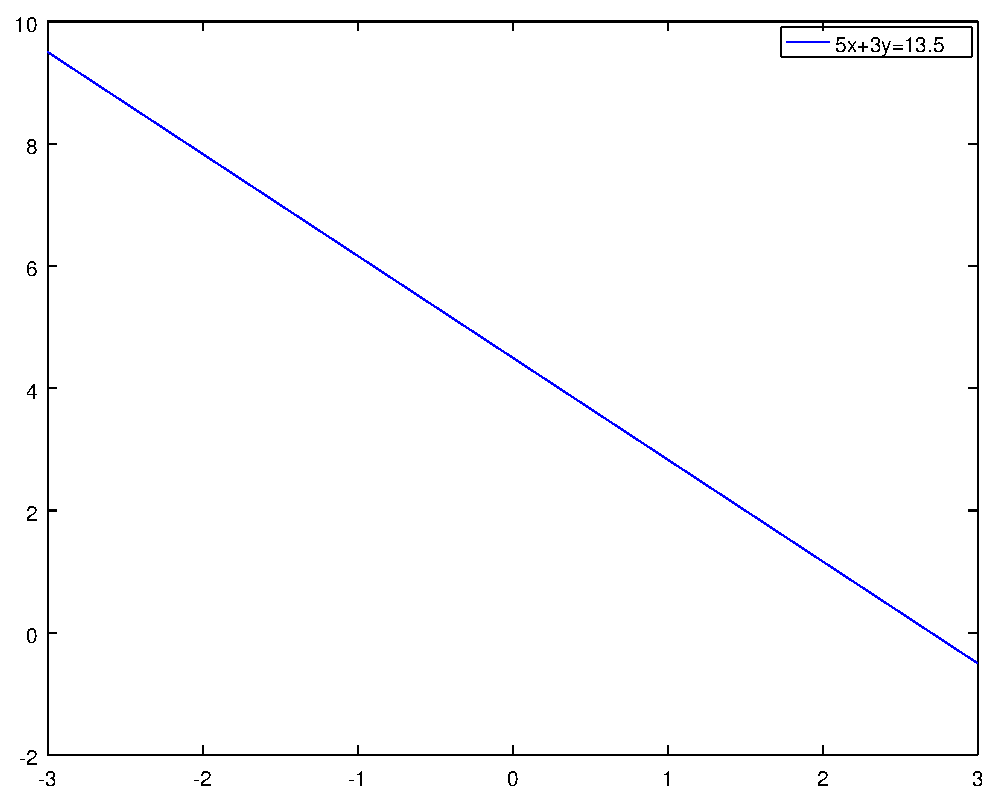
\includegraphics[scale=.6]{./gm-03-SystemsEquations-01.eps}
  \end{figure}
\end{frame}

\begin{frame}
  \frametitle{Graphing Method III}
  \begin{figure}[h]
    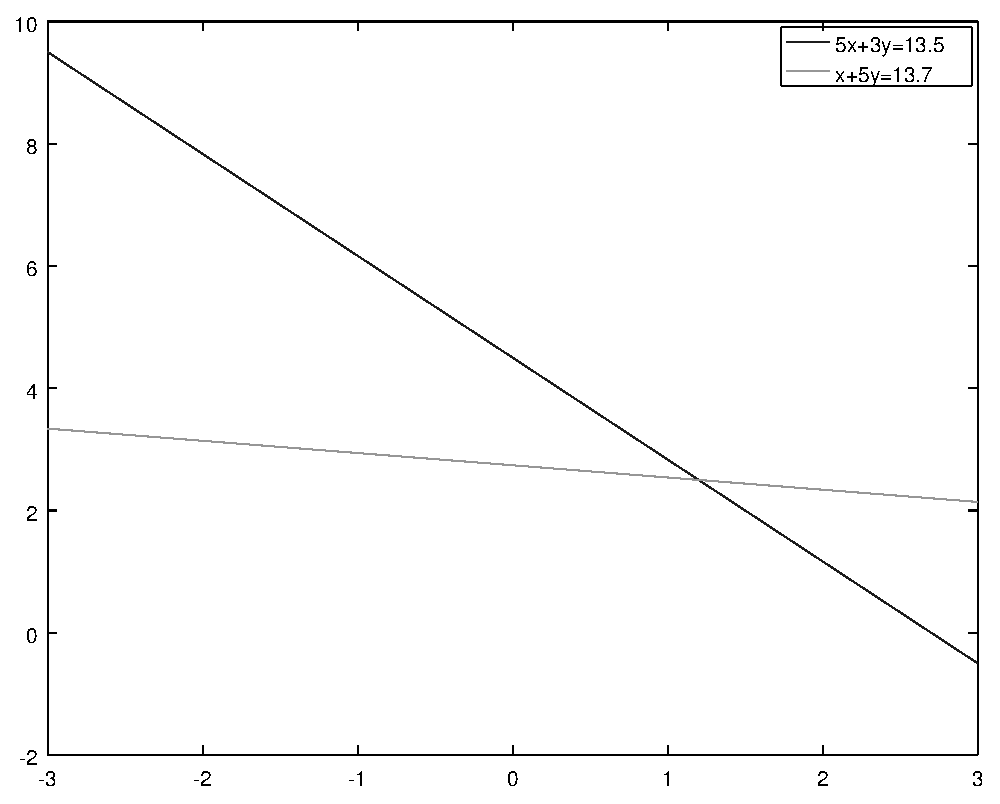
\includegraphics[scale=.6]{./gm-03-SystemsEquations-02.eps}
  \end{figure}
\end{frame}

\begin{frame}
  \frametitle{Graphing Method IV}
  \begin{figure}[h]
    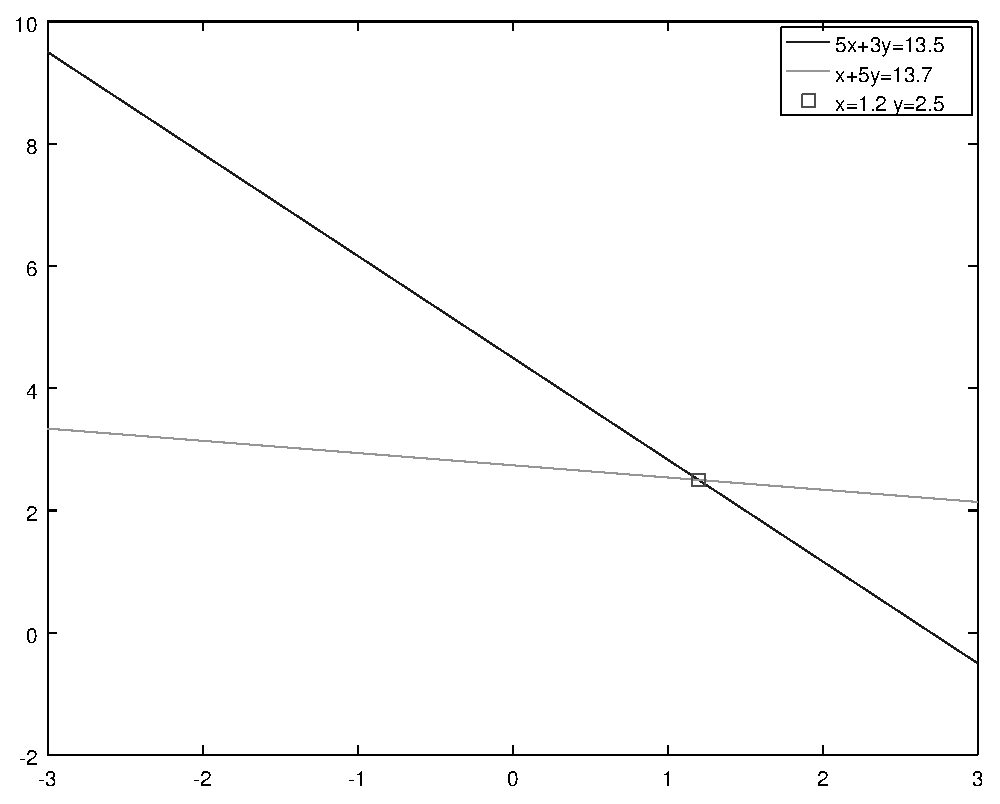
\includegraphics[scale=.6]{./gm-03-SystemsEquations-03.eps}
  \end{figure}
\end{frame}

\begin{frame}
  \frametitle{Graphing Method V}
  \begin{figure}[h]
    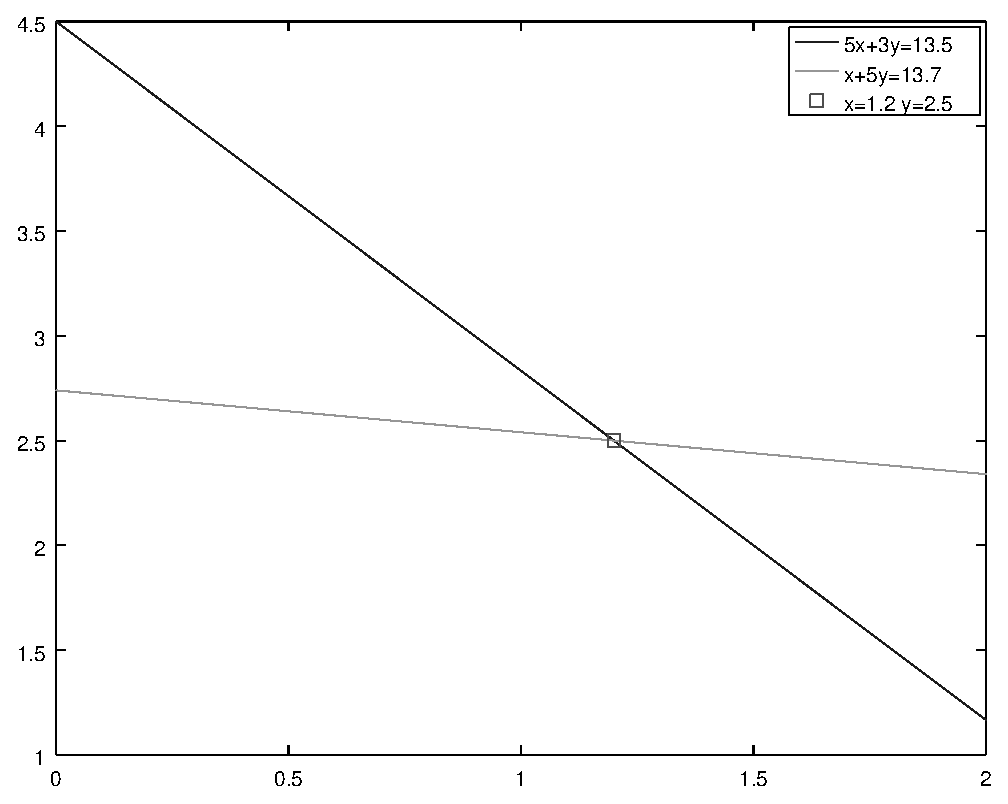
\includegraphics[scale=.6]{./gm-03-SystemsEquations-04.eps}
  \end{figure}
\end{frame}

\begin{frame}
  \frametitle{Graphing Method Exercises}
Find a solution to these systems of linear equations by graphing them
and check your answer by substituting.
  \begin{equation}
    \label{eq:fiesebah}
    \begin{array}{rcrcl}
      7x&-&6y&=&19 \\
      -5x&+&2y&=&-9
    \end{array}
  \end{equation}
  \begin{equation}
    \label{eq:weaseiwa}
    \begin{array}{rcrcl}
      x&+&3y&=&12 \\
      11x&-&2y&=&27
    \end{array}
  \end{equation}
  \begin{equation}
    \label{eq:yaetooni}
    \begin{array}{rcrcl}
      \frac{1}{2}x&-&2y&=&\frac{9}{2} \\
      -\frac{5}{8}x&+&y&=&-\frac{15}{8}
    \end{array}
  \end{equation}
\end{frame}

\begin{frame}
  \frametitle{Substitution Method I}
  \begin{equation}
    \label{eq:jichoora}
    \begin{array}{rcrcl}
      5x&+&3y&=&13.5 \\
      x&+&5y&=&13.7
    \end{array}
  \end{equation}
The second equation yields $x=13.7-5y$. Use this to substitute in the
first equation
  \begin{equation}
    \label{eq:iewoobih}
5\cdot\alert{(13.7-5y)}+3y=13.5
  \end{equation}
therefore, $-22y=-55$ and $y=5/2$. Now substitute $y=5/2$ in the first
equation (you could just as well use the second equation), so
\begin{equation}
  \label{eq:phaiyahj}
  5x+3\cdot\frac{5}{2}=13.5
\end{equation}
which implies $x=1.2$. A banana costs \$1.20; an apple costs \$2.50.
\end{frame}

\begin{frame}
  \frametitle{Substitution Method Exercises}
Find a solution to these systems of linear equations by using the
substitution method.
  \begin{equation}
    \label{eq:waduifee}
    \begin{array}{rcrcl}
      7x&-&6y&=&19 \\
      -5x&+&2y&=&-9
    \end{array}
  \end{equation}
  \begin{equation}
    \label{eq:weiyushe}
    \begin{array}{rcrcl}
      x&+&3y&=&12 \\
      11x&-&2y&=&27
    \end{array}
  \end{equation}
  \begin{equation}
    \label{eq:jiadaush}
    \begin{array}{rcrcl}
      \frac{1}{2}x&-&2y&=&\frac{9}{2} \\
      -\frac{5}{8}x&+&y&=&-\frac{15}{8}
    \end{array}
  \end{equation}
\end{frame}

\begin{frame}
  \frametitle{Elimination Method I}
  \begin{equation}
    \label{eq:ohneirae}
    \begin{array}{rcrcl}
      5x&+&3y&=&13.5 \\
      x&+&5y&=&13.7
    \end{array}
  \end{equation}
is equivalent to
  \begin{equation}
    \label{eq:wahheedo}
    \begin{array}{rcrcl}
      5x&+&3y&=&13.5 \\
      5x&+&25y&=&68.5
    \end{array}
  \end{equation}
\end{frame}

\begin{frame}
  \frametitle{Elimination Method II}
  \begin{equation}
    \label{eq:zeegheir}
    \begin{array}{rcrcl}
      5x&+&3y&=&13.5 \\
      5x&+&25y&=&68.5
    \end{array}
  \end{equation}
implies
  \begin{equation}
    \label{eq:ooleeyae}
(5x+3y)-(5x+25y)=13.5-68.5
  \end{equation}
therefore, $-22y=-55$ and $y=5/2$. Now substitute $y=5/2$ in the first
equation (you could just as well use the second equation), so
\begin{equation}
  \label{eq:ieghoisa}
  5x+3\cdot\frac{5}{2}=13.5
\end{equation}
which implies $x=1.2$. A banana costs \$1.20; an apple costs \$2.50.
\end{frame}

\begin{frame}
  \frametitle{Elimination Method Exercises}
Find a solution to these systems of linear equations by using the
elimination method.
  \begin{equation}
    \label{eq:eighilai}
    \begin{array}{rcrcl}
      7x&-&6y&=&19 \\
      -5x&+&2y&=&-9
    \end{array}
  \end{equation}
  \begin{equation}
    \label{eq:thidaitu}
    \begin{array}{rcrcl}
      x&+&3y&=&12 \\
      11x&-&2y&=&27
    \end{array}
  \end{equation}
  \begin{equation}
    \label{eq:ohkaicux}
    \begin{array}{rcrcl}
      \frac{1}{2}x&-&2y&=&\frac{9}{2} \\
      -\frac{5}{8}x&+&y&=&-\frac{15}{8}
    \end{array}
  \end{equation}
\end{frame}

\begin{frame}
  \frametitle{Matrix Method}
  \begin{equation}
    \label{eq:ohghohfi}
    \begin{array}{rcrcl}
      5x&+&3y&=&13.5 \\
      x&+&5y&=&13.7
    \end{array}
  \end{equation}
is the system of linear equations that we are trying to solve. A
matrix is a rectangular arrangement of numbers, for example
\begin{equation}
  \label{eq:cegeemoi}
  \left[\begin{array}{ccc}
    5&3&13.5 \\
    1&5&13.7
  \end{array}\right]
\end{equation}
There are many fascinating things you can do with matrices. The
discipline that deals with matrices is called Linear Algebra. 
\end{frame}

\begin{frame}
  \frametitle{Matrix Addition}
We can define operations on matrices just like we define operations on
numbers. For example, we can add an $m\times{}n$ matrix to another one
as follows,
\begin{equation}
  \label{eq:ahloongi}
  \left[\begin{array}{cccc}
    a_{11}&a_{12}&\cdots{}&a_{1n} \\
          a_{21}&\ddots{}&& \\
          \vdots{}&&&\vdots \\
          a_{m1}&&\cdots{}&a_{mn}
  \end{array}\right]+\left[
\begin{array}{cccc}
    b_{11}&b_{12}&\cdots{}&b_{1n} \\
          b_{21}&\ddots{}&& \\
          \vdots{}&&&\vdots \\
          b_{m1}&&\cdots{}&b_{mn}
  \end{array}\right]=\notag
\end{equation}
\begin{equation}
  \label{eq:fohghoaw}
\left[
\begin{array}{cccc}
    a_{11}+b_{11}&a_{12}+b_{12}&\cdots{}&a_{1n}+b_{1n} \\
          a_{21}+b_{21}&\ddots{}&& \\
          \vdots{}&&&\vdots \\
          a_{m1}+b_{m1}&&\cdots{}&a_{mn}+b_{mn}
  \end{array}\right]\notag
\end{equation}
\end{frame}

\begin{frame}
  \frametitle{Matrix Scalar Multiplication}
Next, we define what it means to multiply a matrix by a scalar, i.e.\
a real number (NOT a matrix). 
\begin{equation}
  \label{eq:theishie}
  k\cdot\left[\begin{array}{cccc}
    a_{11}&a_{12}&\cdots{}&a_{1n} \\
          a_{21}&\ddots{}&& \\
          \vdots{}&&&\vdots \\
          a_{m1}&&\cdots{}&a_{mn}
  \end{array}\right]=\left[\begin{array}{cccc}
    ka_{11}&ka_{12}&\cdots{}&ka_{1n} \\
          ka_{21}&\ddots{}&& \\
          \vdots{}&&&\vdots \\
          ka_{m1}&&\cdots{}&ka_{mn}
  \end{array}\right]\notag
\end{equation}
\end{frame}

\begin{frame}
  \frametitle{Matrix Product}
Finally, we define matrix multiplication. You can multiply an
$m\times{}j$ matrix by a $j\times{}n$ matrix, which will give you an
$m\times{}n$ matrix.
\begin{equation}
  \label{eq:orahpahn}
  \left[\begin{array}{cccc}
    a_{11}&a_{12}&\cdots{}&a_{1j} \\
          a_{21}&\ddots{}&& \\
          \vdots{}&&&\vdots \\
          a_{m1}&&\cdots{}&a_{mj}
  \end{array}\right]\cdot
\left[\begin{array}{cccc}
    b_{11}&b_{12}&\cdots{}&b_{1n} \\
          b_{21}&\ddots{}&& \\
          \vdots{}&&&\vdots \\
          b_{j1}&&\cdots{}&b_{jn}
  \end{array}\right]=\notag
\end{equation}
\begin{equation}
  \label{eq:raipuboi}
  \left[\begin{array}{cccc}
    c_{11}&c_{12}&\cdots{}&c_{1n} \\
          c_{21}&\ddots{}&& \\
          \vdots{}&&&\vdots \\
          c_{m1}&&\cdots{}&c_{mn}
  \end{array}\right]\notag
\end{equation}
where $c_{ik}=a_{i1}b_{1k}+a_{i2}b_{2k}+\ldots+a_{ij}b_{jk}$.
\end{frame}

\begin{frame}
  \frametitle{Matrix Inverse I}
  Matrix multiplication for an an $m\times{}j$ matrix by a
  $k\times{}n$ matrix is not defined when $j\neq{}k$. An inverse
  matrix $A^{-1}$ of a square matrix $A$ is defined to be the matrix
\begin{equation}
  \label{eq:vaishien}
A\cdot{}A^{-1}=A^{-1}\cdot{}A=E
\end{equation}
where
\begin{equation}
  \label{eq:phoaxoze}
  E=\left[\begin{array}{ccccc}
     1        & 0 & \cdots{} &   & 0      \\
     0        & 1 & \cdots{} &   & 0      \\
     \vdots{} &   & \ddots{} &   & \vdots \\
     0        &   & \cdots{} & 1 & 0      \\
     0        &   & \cdots{} & 0 & 1
  \end{array}\right]\notag
\end{equation}
\end{frame}

\begin{frame}
  \frametitle{Matrices and Systems of Linear Equations I}
Remember our system of linear equations. 
  \begin{equation}
    \label{eq:ahgohcoh}
    \begin{array}{rcrcl}
      5x & + & 3y & = & 13.5 \\
      x  & + & 5y & = & 13.7
    \end{array}
  \end{equation}
In matrix notation, we can write
  \begin{equation}
    \label{eq:neithohn}
  \left[\begin{array}{cc}
5        & 3                 \\
 1       & 5
  \end{array}\right]\cdot
  \left[\begin{array}{c}
 x                 \\
 y
  \end{array}\right]=
  \left[\begin{array}{c}
13.5                 \\
13.7
  \end{array}\right]\notag
  \end{equation}
\end{frame}

\begin{frame}
  \frametitle{Matrices and Systems of Linear Equations II}
Let's call these three matrices $A,v,b$ respectively. $A$ and $b$ are
provided, and we are looking for $v$. If we had $A^{-1}$, we could go
from
\begin{equation}
  \label{eq:baixieda}
  Av=b
\end{equation}
to
\begin{equation}
  \label{eq:maethung}
  A^{-1}Av=A^{-1}b
\end{equation}
which is the same as
\begin{equation}
  \label{eq:leighuga}
  v=A^{-1}b
\end{equation}
The challenge is therefore to find $A^{-1}$. Scientific calculators
and computers can find $A^{-1}$ for you. 
\end{frame}

\begin{frame}
  \frametitle{Matrix Inverse and Determinants}
  If you want to know how to find the inverse yourself, one method to
  use is calculating the determinant of a matrix. It takes a bit of
  time to understand determinants, and then it's still a complicated
  (and not very transparent) procedure to get to the inverse. For
  $2\times{}2$ matrices, however, the inverse is
  \begin{equation}
    \label{eq:iephaizu}
    A^{-1}=\frac{1}{\det{}A}\left[
      \begin{array}{cc}
        d & -b \\
        -c & a
      \end{array}\right]
  \end{equation}
for
  \begin{equation}
    \label{eq:sooxaexa}
    A=\left[
      \begin{array}{cc}
        a & b \\
        c & d
      \end{array}\right]
  \end{equation}
and the determinant is $\det{}A=ad-bc$.
\end{frame}

\begin{frame}
  \frametitle{Matrix Row Operations}
  Another method to find the inverse of a matrix is using
  \alert{matrix row operations}. There are three matrix row
  operations.
\begin{itemize}
\item \alert{Row Switching} means you are allowed to switch two rows,
  for example $R_{1}\leftrightarrow{}R_{2}$
\item \alert{Row Multiplication} means you are allowed to multiply all
  elements of a row by a real non-zero number, for example
  $\frac{2}{5}R_{2}\rightarrow{}R_{2}$
\item \alert{Row Addition} means you are allowed to add one row to
  another and then replace one of the original rows by the sum of the
  two rows, for example $R_{1}+R_{2}\rightarrow{}R_{1}$
\end{itemize}
Row multiplication and row addition are often used together, for
example $\frac{7}{8}R_{1}-R_{3}\rightarrow{}R_{3}$.
\end{frame}

\begin{frame}
  \frametitle{Matrix Row Operations}
To find the inverse of a square matrix, we combine $A$ and $E$
  \begin{equation}
    \label{eq:aurohbac}
  \left[\begin{array}{cccc}
 5 & 3 & 1 & 0 \\
 1 & 5 & 0 & 1
  \end{array}\right]\notag
  \end{equation}
and apply matrix row operations until we get
  \begin{equation}
    \label{eq:nahshooh}
  \left[\begin{array}{cccc}
 1 & 0 & x & y \\
 0 & 1 & z & w
  \end{array}\right]\notag
  \end{equation}
where
  \begin{equation}
    \label{eq:aecocaeh}
  A^{-1}=\left[\begin{array}{cc}
 x & y  \\
 z & w 
  \end{array}\right]\notag
  \end{equation}
\end{frame}

\begin{frame}
  \frametitle{Inverse Example}
For our example,
  \begin{equation}
    \label{eq:weeraesh}
  \left[\begin{array}{cccc}
 5    & 3     & 1     & 0     \\
 1    & 5     & 0     & 1
  \end{array}\right]\longrightarrow
  \left[\begin{array}{cccc}
 25/3 & 5     & 5/3   & 0     \\
 1    & 5     & 0     & 1
        \end{array}\right]\longrightarrow\notag
\end{equation}
  \begin{equation}
  \left[\begin{array}{cccc}
 22/3 & 0     & 5/3   & -1    \\
 1    & 5     & 0     & 1
  \end{array}\right]\longrightarrow\notag
\end{equation}
  \begin{equation}
    \label{eq:ieyoongu}
  \left[\begin{array}{cccc}
 22/3 & 0     & 5/3   & -1    \\
 22/3 & 110/3 & 0     & 22/3
  \end{array}\right]\longrightarrow
  \left[\begin{array}{cccc}
 22/3 & 0     & 5/3   & -1    \\
 0    & 110/3 & -5/3  & 25/3
  \end{array}\right]\longrightarrow\notag
\end{equation}
  \begin{equation}
    \label{eq:ephoopha}
  \left[\begin{array}{cccc}
 1    & 0     & 5/22  & -3/22 \\
 0    & 1     & -1/22 & 5/22
  \end{array}\right]\notag
  \end{equation}
\end{frame}

\begin{frame}
  \frametitle{Inverse Example}
  For step 1, we multiplied the first row by $5/3$ (row
  multiplication). For step 2, we subtracted the second row from the
  first row and replaced the first row by the result (row addition).
  For step 3, we multiplied the second row by $22/3$ (row
  multiplication). For step 4, we subtracted the first row from the
  second row and replaced the second row by the result (row addition).
  For the last step, we multiplied the first row by $3/22$ and the
  second row by $3/110$ (row multiplication applied twice).
\end{frame}

\begin{frame}
  \frametitle{Matrices and Systems of Linear Equations III}
Thus,
\begin{equation}
  \label{eq:oogeujie}
  A^{-1}=\left[\begin{array}{cc}
 5/22  & -3/22 \\
 -1/22 & 5/22
               \end{array}\right]=\frac{1}{22}\cdot\left[
               \begin{array}{cc}
                 5 & -3 \\
                 -1 & 5
               \end{array}\right]\notag
\end{equation}
and
\begin{equation}
  \label{eq:seeleeje}
  v=A^{-1}b=\left[\begin{array}{cc}
 5/22  & -3/22 \\
 -1/22 & 5/22
  \end{array}\right]\cdot
\left[\begin{array}{c}
 13.5   \\
 13.7  
  \end{array}\right]=\left[\begin{array}{c}
 1.2   \\
 2.5  
  \end{array}\right]\notag
\end{equation}
\end{frame}

\begin{frame}
  \frametitle{Professor van Shmowhawk}
  \includemedia[
  width=0.6\linewidth,height=0.45\linewidth,
  activate=pageopen,
  flashvars={
    modestbranding=1 % no YT logo in control bar
   &autohide=1       % controlbar autohide
   &showinfo=0       % no title and other info before start
  }
]{}{https://www.youtube.com/watch?v=ICtDaMWTrrg?rel=0}   % Flash file
\end{frame}

\begin{frame}
  \frametitle{Which Method to Use I}
  The elimination method is usually the fastest. The substitution
  method is most transparent, which means it's easy to see what is
  going on. The substitution method is also helpful for systems of
  equations that are not linear. The matrix method is very powerful
  for systems of equations that have more than two equations. Consider
  this example.
  \begin{equation}
    \label{eq:ohpoongo}
    \begin{array}{rcrcrcrcl}
      5x  & + & 9y & + & 7z & - & 6w & = & -42 \\
      -7x & + & y & - & 9z & + & 9w & = & 38 \\
      -2x & - & 8y & + & 3z & - & 7w & = & -6 \\
      10x & + & 9y & - & 2z & - & 2w & = & -117
    \end{array}
  \end{equation}
\end{frame}

\begin{frame}
  \frametitle{Which Method to Use II}
A computer program tells us that
  \begin{equation}
    \label{eq:iikoquoo}
    \left[\begin{array}{cccc}
        5 & 9    & 7    & -6   \\
       -7 & -1   & -9   & 9    \\
       -2 & -8   & 3    & -7   \\
       10 & 9    & -2   & -2
    \end{array}\right]^{-1}=\frac{1}{4477}\left[\begin{array}{cccc}
-632      & -667 & -379 & 221  \\
572       & 462  & 88   & 55   \\
-79       & -643 & -607 & -532 \\
-507      & -613 & -892 & -354 
    \end{array}\right]\notag
  \end{equation}
and the inverse matrix multiplied by the right-hand side of the system
of equations gives us the solution $x=-5,y=-3,z=10,w=10$.
\end{frame}

\begin{frame}
  \frametitle{Exercises}
  {\ubung} A woman rows a boat upstream from one point on a river to
  another point 4 miles away in 1.5 hours. The return trip, traveling
  with the current, takes only 45 minutes. How fast does she row
  relative to the water, and at what speed is the current flowing?
\end{frame}

\begin{frame}
  \frametitle{Exercises}
  {\ubung} A vintner fortifies wine that contains 10\% alcohol by
  adding 70\% alcohol solution to it. The resulting mixture has an
  alcoholic strength of 16\% and fills 1000 one-litre bottles. How
  many litres of the wine and of the alcoholic solution does she use?
\end{frame}

\begin{frame}
  \frametitle{Exercises}
  {\ubung} Isabella and Wei-Shen leave their house at the same time
  and drive in opposite directions. Isabella drives at 60 kilometres
  an hour and travels 35 kilometres farther than Wei-Shen, who drives
  at 40 kilometres an hour. Wei-Shen's trip takes 15 minutes longer
  than Isabella's. For what length of time does each one of them
  drive?
\end{frame}

\begin{frame}
  \frametitle{Three Variables}
  Solve the following system of linear equations:
  \begin{equation}
    \label{eq:oodaidiz}
    \begin{array}{rcrcrcl}
      -6x&+&&&6z&=&48 \\
      2x&+&5y&-&6z&=&-44 \\
      -3x&+&y&+&2z&=&18 \\
    \end{array}
  \end{equation}
\end{frame}

\begin{frame}
  \frametitle{Three Variables}
  Solve the following system of linear equations:
  \begin{equation}
    \label{eq:ciayamoh}
    \begin{array}{rcl}
      \displaystyle 4y&=&32+5x+6z \\
      && \\
      \displaystyle 7z+5x&=&6y-35 \\
      && \\
      \displaystyle 7y+3z&=&3x-\frac{19}{2} \\
    \end{array}
  \end{equation}
\end{frame}

\begin{frame}
  \frametitle{Solution}
  \begin{equation}
    \label{eq:shuaphai}
    \left[
      \begin{array}{cccccc}
        -5 & 4  & -6 & 1 & 0 & 0 \\
         5 & -6 & 7  & 0 & 1 & 0 \\
        -3 & 7  & 3  & 0 & 0 & 1
      \end{array}\right]\notag
  \end{equation}
  \begin{equation}
    \label{eq:chokishi}
    R_{1}+2\cdot{}R_{3}\longrightarrow{}R_{1}\notag
  \end{equation}
  \begin{equation}
    \label{eq:ahkairoh}
    \left[
      \begin{array}{cccccc}
        -11 & 18  & 0 & 1 & 0 & 2 \\
         5 & -6 & 7  & 0 & 1 & 0 \\
        -3 & 7  & 3  & 0 & 0 & 1
      \end{array}\right]\notag
  \end{equation}
  \begin{equation}
    \label{eq:iejieche}
    R_{2}-\frac{7}{3}\cdot{}R_{3}\longrightarrow{}R_{2}\notag
  \end{equation}
  \begin{equation}
    \label{eq:jineivon}
    \left[
      \begin{array}{cccccc}
        -11 & 18  & 0 & 1 & 0 & 2 \\
         12 & -\frac{67}{3} & 0  & 0 & 1 & -\frac{7}{3} \\
        -3 & 7  & 3  & 0 & 0 & 1
      \end{array}\right]\notag
  \end{equation}
  \begin{equation}
    \label{eq:uamoofuk}
    R_{1}+\frac{11}{12}\cdot{}R_{2}\longrightarrow{}R_{2}\notag
  \end{equation}
\end{frame}

\begin{frame}
  \frametitle{Solution}
  \begin{equation}
    \label{eq:moogiego}
    \left[
      \begin{array}{cccccc}
        -11 & 18  & 0 & 1 & 0 & 2 \\
         12 & -\frac{67}{3} & 0  & 0 & 1 & -\frac{7}{3} \\
        -3 & 7  & 3  & 0 & 0 & 1
      \end{array}\right]\notag
  \end{equation}
  \begin{equation}
    \label{eq:hohpheip}
    R_{1}+\frac{11}{12}\cdot{}R_{2}\longrightarrow{}R_{2}\notag
  \end{equation}
  \begin{equation}
    \label{eq:cahseequ}
    \left[
      \begin{array}{cccccc}
        -11 & 18  & 0 & 1 & 0 & 2 \\
         0 & -\frac{89}{36} & 0  & 1 & \frac{11}{12} & -\frac{5}{36} \\
        -3 & 7  & 3  & 0 & 0 & 1
      \end{array}\right]\notag
  \end{equation}
  \begin{equation}
    \label{eq:kiecaesh}
    R_{1}-\frac{11}{3}\cdot{}R_{3}\longrightarrow{}R_{3}\notag
  \end{equation}
  \begin{equation}
    \label{eq:xeotheem}
    \left[
      \begin{array}{cccccc}
        -11 & 18  & 0 & 1 & 0 & 2 \\
         0 & -\frac{89}{36} & 0  & 1 & \frac{11}{12} & -\frac{5}{36} \\
        0 & -\frac{23}{3}  & -11  & 1 & 0 & -\frac{5}{3}
      \end{array}\right]\notag
  \end{equation}
  \begin{equation}
    \label{eq:ioquooxa}
    36\cdot{}R_{2}\longrightarrow{}R_{2}\hspace{.5in}3\cdot{}R_{3}\longrightarrow{}R_{3}\notag
  \end{equation}
\end{frame}

\begin{frame}
  \frametitle{Solution}
  \begin{equation}
    \label{eq:viedixee}
    \left[
      \begin{array}{cccccc}
        -11 & 18  & 0 & 1 & 0 & 2 \\
         0 & -\frac{89}{36} & 0  & 1 & \frac{11}{12} & -\frac{5}{36} \\
        0 & -\frac{23}{3}  & -11  & 1 & 0 & -\frac{5}{3}
      \end{array}\right]\notag
  \end{equation}
  \begin{equation}
    \label{eq:laiwoami}
    36\cdot{}R_{2}\longrightarrow{}R_{2}\hspace{.5in}3\cdot{}R_{3}\longrightarrow{}R_{3}\notag
  \end{equation}
  \begin{equation}
    \label{eq:huajahng}
    \left[
      \begin{array}{cccccc}
        -11 & 18  & 0 & 1 & 0 & 2 \\
         0 & -89 & 0  & 36 & 33 & -5 \\
        0 & -23  & -33  & 3 & 0 & -5
      \end{array}\right]\notag
  \end{equation}
  \begin{equation}
    \label{eq:naesahto}
R_{2}+\frac{89}{18}\cdot{}R_{1}\longrightarrow{}R_{1}\notag    
  \end{equation}
  \begin{equation}
    \label{eq:yohteihu}
    \left[
      \begin{array}{cccccc}
        -\frac{979}{18} & 0  & 0 & \frac{737}{18} & 33 & \frac{88}{18} \\
         0 & -89 & 0  & 36 & 33 & -5 \\
        0 & -23  & -33  & 3 & 0 & -5
      \end{array}\right]\notag
  \end{equation}
  \begin{equation}
    \label{eq:ajiuteeb}
R_{2}-\frac{89}{23}\cdot{}R_{3}\longrightarrow{}R_{3}\hspace{.5in}18\cdot{}R_{1}\longrightarrow{}R_{1}\notag     
  \end{equation}
\end{frame}

\begin{frame}
  \frametitle{Solution}
  \begin{equation}
    \label{eq:aichohmi}
    \left[
      \begin{array}{cccccc}
        -\frac{979}{18} & 0  & 0 & \frac{737}{18} & 33 & \frac{88}{18} \\
         0 & -89 & 0  & 36 & 33 & -5 \\
        0 & -23  & -33  & 3 & 0 & -5
      \end{array}\right]\notag
  \end{equation}
  \begin{equation}
    \label{eq:opahyahs}
R_{2}-\frac{89}{23}\cdot{}R_{3}\longrightarrow{}R_{3}\hspace{.5in}18\cdot{}R_{1}\longrightarrow{}R_{1}\notag     
  \end{equation}
  \begin{equation}
    \label{eq:chahtiye}
    \left[
      \begin{array}{cccccc}
        -979 & 0  & 0 & 737 & 594 & 88 \\
         0 & -89 & 0  & 36 & 33 & -5 \\
        0 & 0  & \frac{2937}{23}  & \frac{561}{23} & 33 & \frac{330}{23}
      \end{array}\right]\notag
  \end{equation}
  \begin{center}
    clean up
  \end{center}
  \begin{equation}
    \label{eq:thuoxook}
    A^{-1}=\frac{1}{89}\left[
      \begin{array}{ccc}
     -67&-54&-8 \\
        -36&-33&5 \\
        17&23&10
      \end{array}\right]\notag
  \end{equation}
\end{frame}

\begin{frame}
  \frametitle{Solution}
  The solution vector for the system of linear equations is
  \begin{equation}
    \label{eq:chiesooh}
    v=A^{-1}\cdot{}b=\frac{1}{89}\cdot\left[
      \begin{array}{ccc}
     -67&-54&-8 \\
        -36&-33&5 \\
        17&23&10
      \end{array}\right]
    \left[
      \begin{array}{c}
     32 \\
     -35 \\
     -\frac{19}{2}
      \end{array}\right]=
    \left[
      \begin{array}{c}
     -2 \\
     -\frac{1}{2} \\
     -4
      \end{array}\right]\notag
  \end{equation}
Therefore, $S=\{(-2,-\frac{1}{2},-4)\}$. Note that it is sometimes
difficult to keep zeros you already have in place when you do elementary
row operations. The trick is that when you are trying to get a second
zero in a row, you must do this with another row that shares the first
row's first zero. For example, use row 1 and row 3 to get a zero in
row 1's third place. Then use row 2 and row 3 to get a zero in
row 2's third place. Now you have a zero both in row 1's third place
and in row 2's third place, so you can use row 1 and row 2 to get
another zero in row 1's second place without losing the zero that is
already in third place.
\end{frame}

\begin{frame}
  \frametitle{Fruit in a Bag}
  You have a cone shaped bag. At the bottom of the bag is an orange
  with a radius of 2 inches. On top of the orange is a melon with a
  radius of 6 inches. It touches the orange and fits snugly in the
  bag, touching it in a ring around the orange. Its top is at the same
  level as the top of the bag. Calculate the height of the cone.
  \begin{figure}[h]
    \includegraphics[scale=.4]{./p82.png}
  \end{figure}
\end{frame}

\begin{frame}
  \frametitle{Exercises}
{\ubung} Solve the following system of equations,
\begin{equation}
  \label{eq:texeewok}
  \begin{array}{rcrcl}
\frac{x}{3}   & + & \frac{y}{2} & = & \frac{4}{3} \\ 
\hspace{.1in} &   &             &   &             \\
\frac{x}{2}   & + & \frac{y}{3} & = & \frac{7}{6}
  \end{array}
\end{equation}
\end{frame}

\begin{frame}
  \frametitle{Exercises}
{\ubung} Find the inverse of the following matrix. Show your work (i.e.\
the elementary row operations).
\begin{equation}
  \label{eq:uquuacha}
  \left[\begin{array}{cc}
    3 & 6 \\
   -7 & 1
  \end{array}\right]
\end{equation}
\end{frame}

\begin{frame}
  \frametitle{End of Lesson}
Next Lesson: The Right Triangle.
\end{frame}

\end{document}

